
%%%%%%%%%%%%%%%%%%%%%%%%%%%%%%%%%%%%%%%%%%%%%%%%%%%%%%%%%%%%%%%%%%%%%%%%%%%%%%
% Copyright (c) 2003-2016 by The University of Queensland
% http://www.uq.edu.au
%
% Primary Business: Queensland, Australia
% Licensed under the Open Software License version 3.0
% http://www.opensource.org/licenses/osl-3.0.php
%
% Development until 2012 by Earth Systems Science Computational Center (ESSCC)
% Development 2012-2013 by School of Earth Sciences
% Development from 2014 by Centre for Geoscience Computing (GeoComp)
%
%%%%%%%%%%%%%%%%%%%%%%%%%%%%%%%%%%%%%%%%%%%%%%%%%%%%%%%%%%%%%%%%%%%%%%%%%%%%%%


\section{Some Remarks on Lumping}
\label{LUMPING}

Explicit time integration schemes (two examples are discussed later in this 
section), require very small time steps in order to maintain numerical stability. 
Unfortunately, these small time increments often result in a prohibitive 
computational cost. 
In order to minimise these costs, a technique termed lumping can be utilised.
Lumping is applied to the coefficient matrix, reducing it to a simple diagonal 
matrix. This can significantly improve the computational speed, because the 
solution updates are simplified to a simple component-by-component 
vector-vector product. However, some care is required when making radical
approximations such as these. In this section, two commonly applied lumping
techniques are discussed, namely row sum lumping 
\index{linear solver!row sum lumping}\index{row sum lumping}and HRZ 
lumping\index{linear solver!HRZ lumping}\index{HRZ lumping}.

\subsection{Scalar wave equation}
One example where lumping can be applied to a hyperbolic problem, is  
the scalar wave equation
\begin{eqnarray} \label{LUMPING WAVE} 
u_{,tt}=c^2 u_{,ii} \; .
\end{eqnarray}
In this example, both of the lumping schemes are tested against the reference solution
\begin{eqnarray} \label{LUMPING WAVE TEST} 
u=sin(5 \pi (x_0-c*t) )
\end{eqnarray}
over the 2D unit square. Note that $u_{,i}n_i=0$ on faces $x_1=0$ and $x_1=1$.
Thus, on the faces $x_0=0$ and $x_0=1$ the solution is constrained.

To solve this problem the explicit Verlet scheme\index{Verlet scheme} was used 
with a constant time step size $dt$ given by 
\begin{eqnarray} \label{LUMPING WAVE VALET}
u^{(n)}=2u^{(n-1)}-u^{(n-2)} + dt^2 a^{(n)}
\end{eqnarray}
for all $n=2,3,\ldots$ where the upper index ${(n)}$ refers to values at 
time $t^{(n)}=t^{(n-1)}+h$ and $a^{(n)}$ is the solution of 
\begin{eqnarray} \label{LUMPING WAVE VALET 2} 
a^{(n)}=c^2 u^{(n-1)}_{,ii} \; .
\end{eqnarray}
This equation can be interpreted as a PDE for the unknown value $a^{(n)}$,
which must be solved at each time-step. 
In the notation of equation~\ref{LINEARPDE.SINGLE.1} we thus set $D=1$ and 
$X=-c^2 u^{(n-1)}_{,i}$. Furthermore, in order to maintain stability, 
the time step size needs to fulfill the Courant-Friedrichs-Lewy condition 
(CFL condition).
\index{Courant condition}
\index{explicit scheme!Courant condition} 
For this example, the CFL condition takes the form 
\begin{eqnarray} \label{LUMPING WAVE CFL} 
dt = f \cdot \frac{dx}{c} .
\end{eqnarray}
where $dx$ is the mesh size and $f$ is a safety factor. In this example, 
we use $f=\frac{1}{6}$.

Figure~\ref{FIG LUMPING VALET A} depicts a temporal comparison between four 
alternative solution algorithms: the exact solution; using a full mass matrix;
using HRZ lumping; and row sum lumping. The domain utilised rectangular order 1 
elements (element size is $0.01$) with observations taken at the point 
$(\frac{1}{2},\frac{1}{2})$. 
All four solutions appear to be identical for this example. This is not the case
for order $2$ elements, as illustrated in Figure~\ref{FIG LUMPING VALET B}.
For the order $2$ elements, the row sum lumping has become unstable. Row sum
lumping is unstable in this case because for order $2$ elements, a row sum can 
result in a value of zero. HRZ lumping does not display the same problems, but 
rather exhibits behaviour similar to the full mass matrix solution. When using
both the HRZ lumping and full mass matrix, the wave-front is slightly delayed 
when compared with the analytical solution.

\begin{figure}[ht]
\centerline{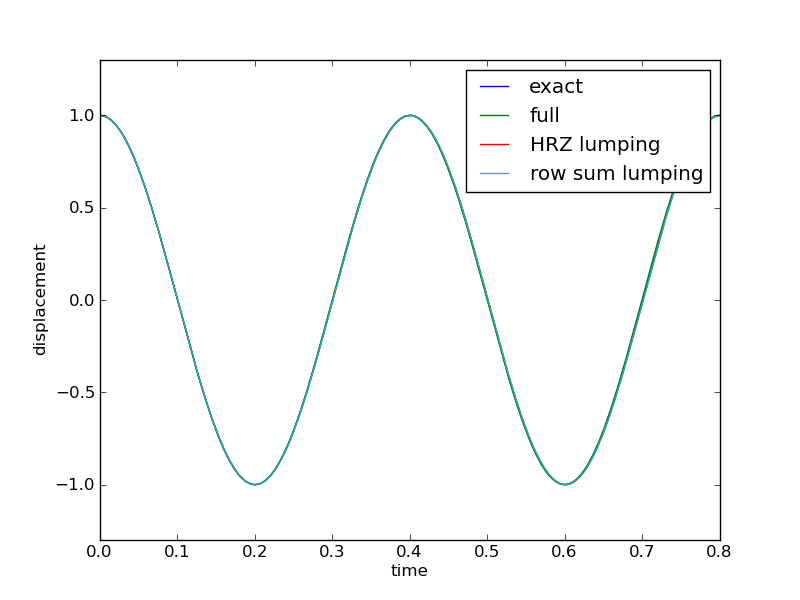
\includegraphics[width=7cm]{lumping_valet_a_1}}
\caption{Amplitude at point $(\frac{1}{2},\frac{1}{2})$ using the acceleration formulation~\ref{LUMPING WAVE VALET 2} of the 
Velet scheme with order $1$ elements, element size $dx=0.01$, and $c=1$.}
\label{FIG LUMPING VALET A}
\end{figure}

\begin{figure}[ht]
\centerline{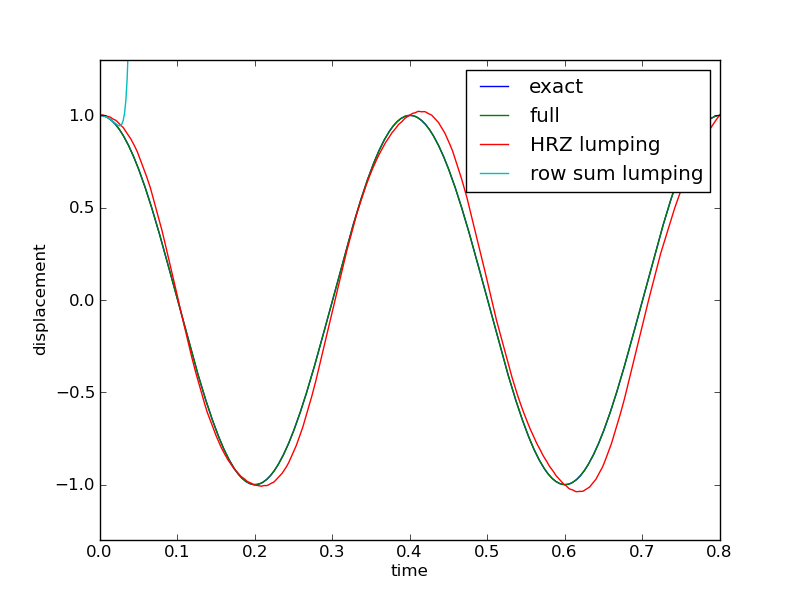
\includegraphics[width=7cm]{lumping_valet_a_2}}
\caption{Amplitude at point $(\frac{1}{2},\frac{1}{2})$ using the acceleration formulation~\ref{LUMPING WAVE VALET 2} of the 
Velet scheme with order $2$ elements, element size $0.01$, and $c=1$.}
\label{FIG LUMPING VALET B}
\end{figure}

\begin{figure}[ht]
\centerline{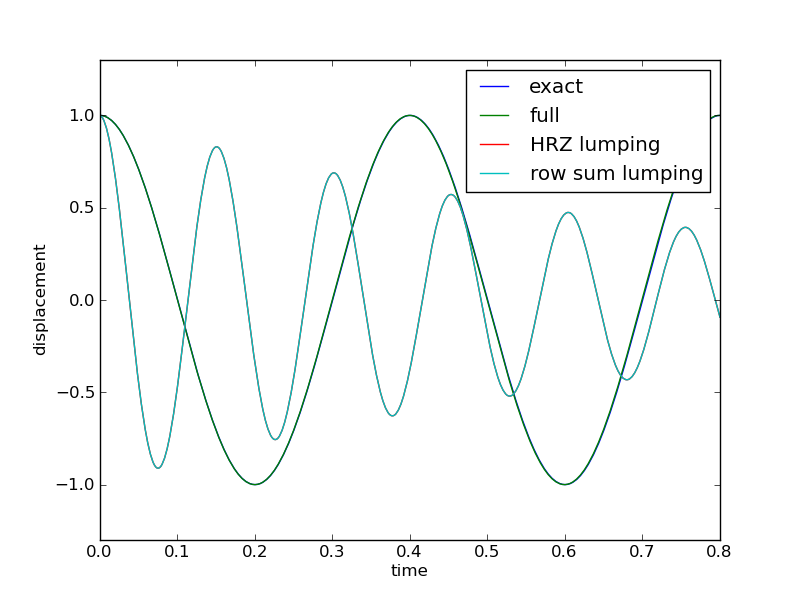
\includegraphics[width=7cm]{lumping_valet_u_1}}
\caption{Amplitude at point $(\frac{1}{2},\frac{1}{2})$ using the displacement formulation~\ref{LUMPING WAVE VALET 3} of the 
Velet scheme with order $1$ elements, element size $0.01$ and $c=1$.}
\label{FIG LUMPING VALET C}
\end{figure}

Alternatively, one can directly solve for $u^{(n)}$ by inserting 
equation~\ref{LUMPING WAVE VALET} into equation~\ref{LUMPING WAVE VALET 2}:
\begin{eqnarray} \label{LUMPING WAVE VALET 3} 
u^{(n)}=2u^{(n-1)}-u^{(n-2)} + (dt\cdot c)^2 u^{(n-1)}_{,ii} \; .
\end{eqnarray}
This can also be interpreted as a PDE that must be solved at each time-step, but 
for the unknown $u^{(n)}$. 
As per equation~\ref{LINEARPDE.SINGLE.1} we set the general form coefficients to:
$D=1$; $Y=2u^{(n-1)}-u^{(n-2)}$; and $X=-(h\cdot c)^2 u^{(n-1)}_{,i}$. 
For the full mass matrix, the acceleration ~\ref{LUMPING WAVE VALET 2} and displacement formulations ~\ref{LUMPING WAVE VALET 3}
are identical. 

The displacement solution is depicted in Figure~\ref{FIG LUMPING VALET C}. The
domain utilised order $1$ elements (for order $2$, both 
lumping methods are unstable). The solutions for the exact and the full mass 
matrix approximation are almost identical while the lumping solutions, whilst 
identical to each other, exhibit a considerably faster wave-front propagation 
and a decaying amplitude.

\subsection{Advection equation}
Consider now, a second example that demonstrates the advection equation
\begin{eqnarray} \label{LUMPING ADVECTIVE} 
u_{,t}=(v_i u)_i \; .
\end{eqnarray}
where $v_i$ is a given velocity field. To simplify this example, set $v_i=(1,0)$ and
\begin{equation} \label{LUMPING ADVECTIVE TEST} 
u(x,t)= 
\left\{
   \begin{array}{cl}
   1 &  x_0 < t \\
   0 &  x_0 \ge t 
   \end{array}
\right\}.
\end{equation}
The solution scheme implemented, is the two-step Taylor-Galerkin scheme 
\index{Taylor-Galerkin scheme}
(which is in this case equivalent to SUPG\index{SUPG}):
the incremental formulation is given as
\begin{eqnarray} \label{LUMPING SUPG 1} 
du^{(n-\frac{1}{2})} = \frac{dt}{2} (v_i u^{(n-1)})_i \\
du^{(n)} = dt (v_i (u^{(n-1)}+du^{(n-\frac{1}{2})}) )_i \\
u^{(n)} = u^{(n)} + du^{(n)} 
\end{eqnarray}
This can be reformulated to calculate $u^{(n)}$ directly:
\begin{eqnarray} \label{LUMPING SUPG 2} 
u^{(n-\frac{1}{2})} = u^{(n-1)} + \frac{dt}{2} (v_i u^{(n-1)})_i \\
u^{(n)} =  u^{(n-1)} + dt (v_i u^{(n-\frac{1}{2})} )_i 
\end{eqnarray}
In some cases it may be possible to combine the two equations to calculate 
$u^{(n)}$ without the intermediate step. This approach is not discussed, because
 it is inflexible when a greater number of terms (e.g. a diffusion term) are
 added to the right hand side. 

The advection problem is thus similar to the wave propagation problem, because 
the time step also needs to satisfy the CFL condition
\index{Courant condition}\index{explicit scheme!Courant condition}. For the 
advection problem, this takes the form
\begin{eqnarray} \label{LUMPING ADVECTION CFL} 
dt = f \cdot \frac{dx}{\|v\|} .
\end{eqnarray}
where $dx$ is the mesh size and $f$ is a safty factor. 
For this example, we again use $f=\frac{1}{6}$.

Figures~\ref{FIG LUMPING SUPG INC A} and~\ref{FIG LUMPING SUPG INC B} illustrate
the four incremental formulation solutions: the true solution; the exact mass matrix;
the HRZ lumping; and the row sum lumping. Observe, that for the order $1$ elements
case, there is little deviation from the exact solution before the wave front,
whilst there is a significant degree of osciallation after the wave-front has 
passed. For the order $2$ elements example, all of the numerical techniques fail. 

\begin{figure}[ht]
\centerline{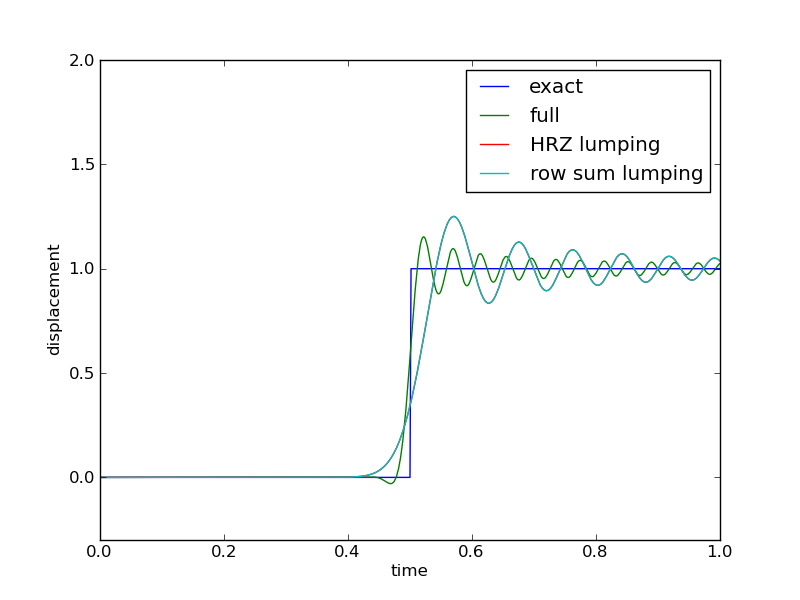
\includegraphics[width=7cm]{lumping_SUPG_du_1}}
\caption{Amplitude at point $(\frac{1}{2},\frac{1}{2})$ using the incremental formulation~\ref{LUMPING SUPG 1} of the 
Taylor-Galerkin scheme with order $1$ elements, element size $dx=0.01$, $v=(1,0)$.}
\label{FIG LUMPING SUPG INC A}
\end{figure}

\begin{figure}[ht]
\centerline{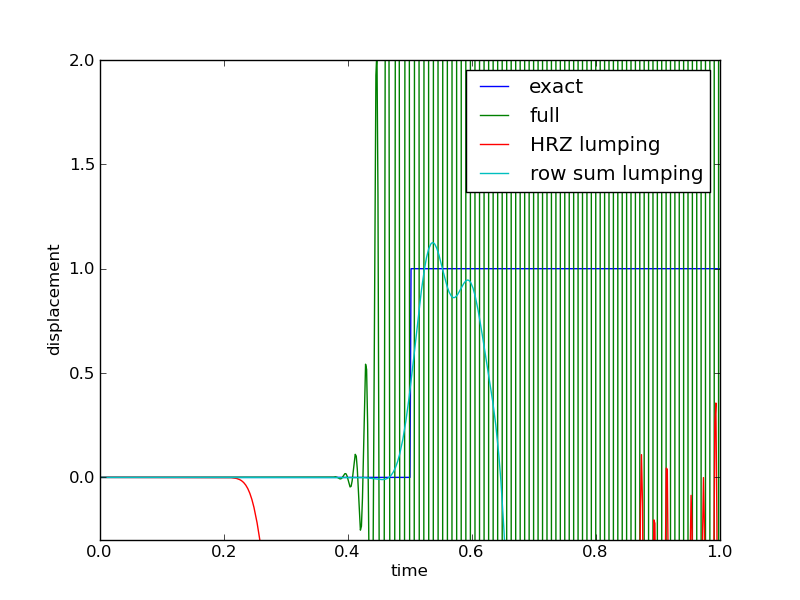
\includegraphics[width=7cm]{lumping_SUPG_du_2}}
\caption{Amplitude at point $(\frac{1}{2},\frac{1}{2})$ using the incremental formulation~\ref{LUMPING SUPG 1} of the 
Taylor-Galerkin scheme  with order $2$ elements, element size $0.01$, $v=(1,0)$.}
\label{FIG LUMPING SUPG INC B}
\end{figure}

Figure~\ref{FIG LUMPING SUPG A} depicts the results from the direct formulation
of the advection problem for an order $1$ mesh. Generally, the results have
improved when compared with the incremental formulation. The full mass matrix 
still introduces some osciallation both before and after the arrival of the 
wave-front at the observation point. The two lumping solutions are identical, and
have introduced additional smoothing to the solution. There are no oscillatory
effects when using lumping for this example. In Figure~\ref{FIG LUMPING SUPG Ab}
the mesh or element size has been reduced from 0.01 to 0.002 units. As predicted
by the CFL condition, this significantly improves the results when lumping is 
applied. However, when utilising the full mass matrix, a smaller mesh size will 
result in post wave-front oscilations which are higher frequency and slower to 
decay.

Figure~\ref{FIG LUMPING SUPG B} illustrates the results when utilising elements 
of order $2$. The full mass matrix and HRZ lumping formulations are unable to 
correctly model the exact solution. Only the row sum lumping was capable of 
producing a smooth and sensical result. 

\begin{figure}[ht]
\centerline{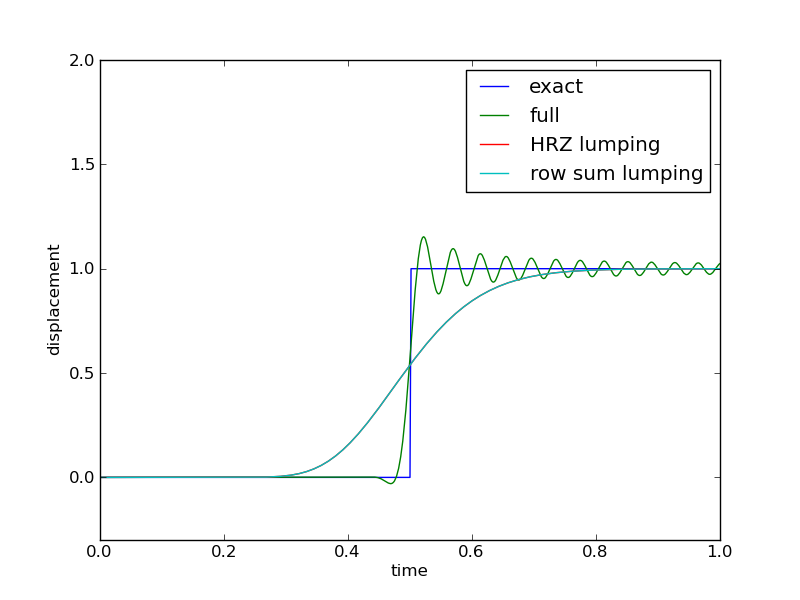
\includegraphics[width=7cm]{lumping_SUPG_u_1}}
\caption{Amplitude at point $(\frac{1}{2},\frac{1}{2})$ using the direct formulation~\ref{LUMPING SUPG 2} of the 
Taylor-Galerkin scheme using order $1$ elements, element size $dx=0.01$, $v=(1,0)$.}
\label{FIG LUMPING SUPG A}
\end{figure}

\begin{figure}[ht]
\centerline{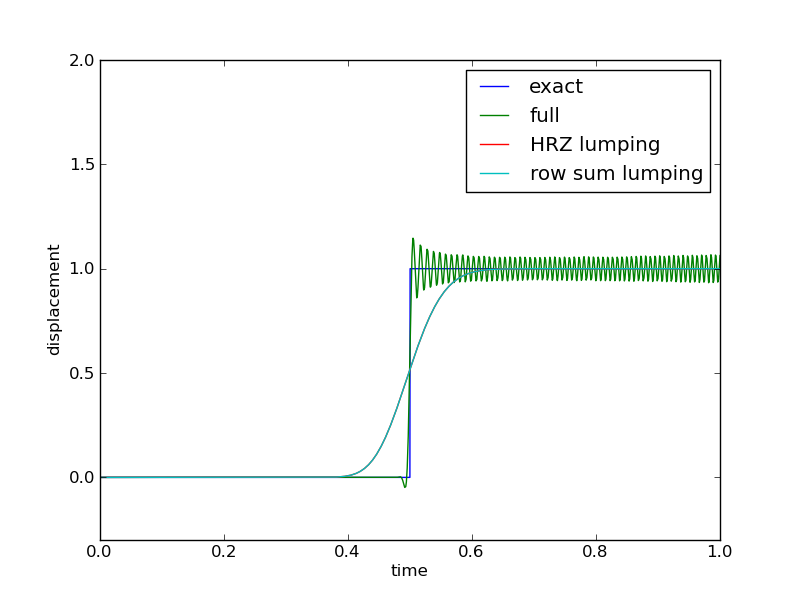
\includegraphics[width=7cm]{lumping_SUPG_u_1b}}
\caption{Amplitude at point $(\frac{1}{2},\frac{1}{2})$ using the direct formulation~\ref{LUMPING SUPG 2} of the 
Taylor-Galerkin scheme using order $1$ elements, element size $dx=0.002$, $v=(1,0)$.}
\label{FIG LUMPING SUPG Ab}
\end{figure}

\begin{figure}[ht]
\centerline{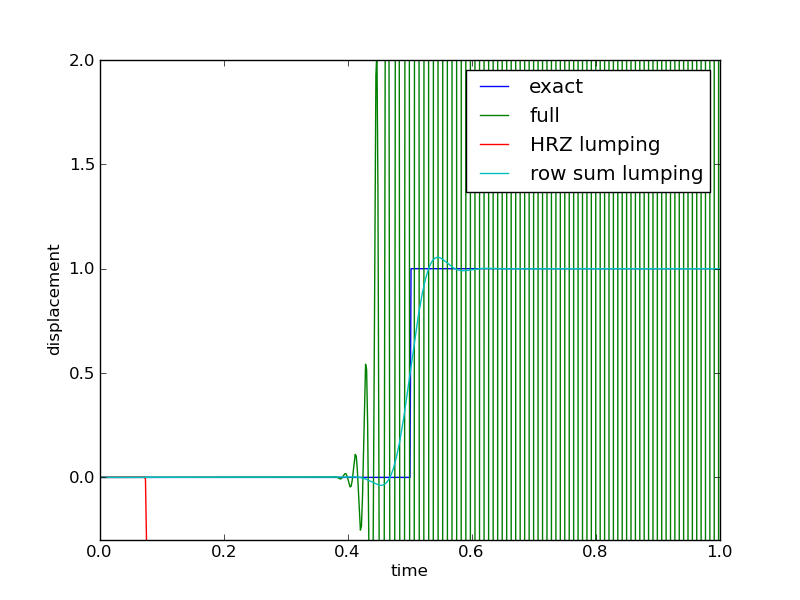
\includegraphics[width=7cm]{lumping_SUPG_u_2}}
\caption{Amplitude at point $(\frac{1}{2},\frac{1}{2})$ using the direct formulation~\ref{LUMPING SUPG 2} of the 
Taylor-Galerkin scheme  using order $2$ elements, element size $0.01$, $v=(1,0)$.}
\label{FIG LUMPING SUPG B}
\end{figure}

\subsection{Summary}
The examples in this section have demonstrated the capabilities and limitations
of both HRZ and row sum lumping with comparisons to the exact and full mass 
matrix solutions. Wave propagation type problems that utilise lumping, produce 
results simular the full mass matrix at significantly 
lower computation cost. An acceleration based formulation, with HRZ lumping 
should be implemented for such problems, and can be applied to both order $1$ and
 order $2$ elements. 

In transport type problems, it is essential that row sum lumping is used to 
achieve a smooth solution. Additionally, it is not recommended that second order
elements be used in advection type problems.



